\documentclass[a4paper,10pt]{article}
\usepackage[catalan]{babel}
\usepackage[utf8x]{inputenc}
\usepackage{amsmath}
\usepackage{amsfonts}
\usepackage{amssymb}
\usepackage{amsthm}
\usepackage{graphicx}


\title{Memòria pràctica 8}
\author{Josep Marc Mingot//, 
      Gabriel Reines}
      
%%%%%%%%%%%%%%%%%%%%%%%%%%%%%%%%%%%%%%%%%%%%%%%%%%%%%%%%%%%%%%%%%%%%%%%%%%%%%%%%%%%%%%%%%%%%%%%%%%%
\usepackage{Sweave}
\begin{document}

\Sconcordance{concordance:memoria.tex:memoria.Rnw:%
1 15 1 1 0 1 4 34 1 1 4 6 1 1 4 38 1 1 2 15 0 1 2 15 1 1 2 16 0 1 2 1 1 1 5 6 1 1 4 6 1 1 4 25 1 1 4 6 1 1 4 6 1 1 4 40 1}



\maketitle

\begin{abstract}
\end{abstract}

\newpage
\tableofcontents

\newpage
%%%%%%%%%%%%%%%%%%%%%%%%%%%%%%%%%%%%%%%%%%%%%%%%%%%%%%%%%%%%%%%%%%%%%%%%%%%%%%%%%%%%%%%%%%%%%%%%%%%
\section{Introducció}

[Explicació del problema i lllista de variables a usar.]
La KDD Cup és una competició anual de Mineria de Dades organitzada per l'ACM (Special Interest Group on Knowledge Discovery and Data Mining). Cada any milers d'equips de tot el món competeixen per donar solució a un problema de mineria de dades patrocinat per una empresa o organització. En aquest treball ens hem plantejat donar una solució al problema plantejat per la KDD Cup del 2006, patrocinada per la Universitat de Nuevo Méjico.
\\
\\
El problema que és va plantejar en aquesta edició consistia en la detecció de embolies pulmonars (PE) a través de dades extretes de un CAD 3-d del pacient. Les PE ocurreixen quan una artèria del pulmó queda obstruida. Malgrat que aquesta obstrucció molts cops no és letal, és la tercera causa més comuna de morta als EUA amb almenys 65000 casos cada any. El repte està en poder diagnosticar al pacient el més aviat possible. Això no obstant no és gens senzill ja que els símptomes dels PE són molt pareguts a altres patologies molt comunes. Per detectar PE una tècnica molt recent és l'anomenada CTA (Computed Tomography Angiography) que consisteix en pendre moltes imatges dels pulmons cada una de elles representant una secció del pulmó. Aquestes imatges són processades computacionalment per extreure'n de cada una una variables i \textit{candidats} a PE. Entenem per candidat a aquell punt del pulmó que pot ser un PE (encara que també podria ser altres artifactes del pulmó). El repte consisteix en classificar els PE donades un conjunt de variables ja extretes de les imatges.
\\
\\
La base de dades està formada per 38 pacients positius i 8 negatius. En total tots aquests pacients donen lloc a 3038 candidats a PE que són les files de la nostra base dedades. Cada candidat conté 116 variables extretes de les imatges de CAD dels pulmons. Les tres primeres variables són les coordenades $x$, $y$ i $z$ del candidat. La resta de variables poden ser dividides en 3 grups: aquelles que corresponen a la distribució d'intensitat dels voxels que formen el candidat, les distribucions d'intensitat dels voxels del voltant del candidat i les que descriuen la forma 3-D.
\\
\\
Finalment fem un breu incís sobre el marc de treball que hem configurat per avaluar els classificadors. Hem dividit les dades en un conjunt d'entrenament (70\%) i un de test (30\%). El conjunt de test és l'usat per avaluar l'error en els classificadors. En alguns casos s'ha usat la tècnica de la validació creuada \textit{k-fold} per donar més robustesa a les estimacions de l'error. En ells, s'ha dividit el conjunt de dades en 5 grups: 4 s'han usat per entrenar i 1 per avaluar donant un total de 5 mesures de l'error. Finalment per avaluar l'error dels classificadors usem 2 mpetriques diferents. La probabilitat d'error directament sobre el conjunt de test i l'àrea sota la curva ROC (AUC). La diferència princpial entre aquestes dos mètriques és que mentre la primera ens diu la probabilitat de classificar un candidat aleatori com a correcte, la segona ens estima la probabilitat de classificar un candidat positiu aleatori com a correcte. En aquest sentit l'AUC ens dona una mesura més robusta que la probabilitat d'error en conjunts no balancejats.


%%%%%%%%%%%%%%%%%%%%%%%%%%%%%%%%%%%%%%%%%%%%%%%%%%%%%%%%%%%%%%%%%%%%%%%%%%%%%%%%%%%%%%%%%%%%%%%%%%%
\section{Visualització de dades}

El primer pas en qualsevol problema de classificació és entendre les dades que se'ns han donat: realació entre les diferents variables, rànking de quines són potencialment més importants i distribucions d'aquestes. Per aquest motiu en aquesta secció pretenem donar a través de l'anàlisi visual, una serie de propietats sobre les variables que influeixen en el problema.
\\
\\
Comencem estudiant la correlació entre elles. Al tenir 116 variables l'eina més adequada per visualitzar l'autocorrelació entre elles és plasmar gràficament la matriu de correlació. En la figura \ref{fig:autoc} observem la matriu on cada casella representa un valor de la matriu i com més fosc més proper a 1. Hi ha variables que estan completament correlacionades (per exemple \texttt{neighborhood intensity feature 2} amb \texttt{neighborhood intensity feature 8}). Per eliminar-les, fixem un nivell a partir del qual considerem que les variables estan correlacionades i n'eliminem aquella que té una mitja de correlació més alta amb les altres. Després d'aquest procés i fixant un tall a 0.85 passem de 116 variables a 91 variables. Podem observar la matriu d'autocorrelació neta en la figura \ref{fig:autoc_clean}.
\\
\\
Després de netejar les variables autocorrelacionades, fem un anàlisi exploratòria d'algunes variables. De les variables ens interessa coneixer la seva distribució condicionada a la classe, boxplots segons classe, scatter plots 2 a 2 amb altres variables (per veure possibles parelles de variables que separin). Podem obtenir tots aquests descriptius de les variables en una sola imatge. En la figura \ref{fig:pos} observem aquests descriptius per les variables de posició (coordenades x,y i z del PE) i la mida del PE candidat (amb el nom de \texttt{V5}). Observem com l'\textit{scatter} de les coordenades de posició ens dibuixen els plans de tall d'uns pulmons com calia esperar. Tanmateix observem també que no és descriminador la posició del candidat per dir si és o no PE. Respecte a la variable "mida" si que veiem que és més discriminador: els scatters amb les coordenades ens consegueixen separar prou bé els 1 dels 0. 
\\
\\
Finalment en la figura \ref{fig:top_var} podem observar els mateixos descriptius comentats anteriorment per a les 7 variables més significatives del model segons el \textit{CAT score} (ja en donarem més detalls en l'apartat LDA). Observem per anàlisis visual que cap de les distribucions condicionades (primera columna de la imatge) s'acosta a una distribució gaussiana, però les distribucions condicionades a les classes són diferents (no s'acaba de poder apreciar ja que motrem la freqüència enlloc de la densitat). Per altra banda, els boxplots condicionats (primera fila) en mostra com efectivament ens donen distribucions diferents segons la classe. Com més diferents siguin les distribucions condicionades a la classe més senzill en serà poder separar (no en va estem mostrant aquí les nostres top 7 variables). 



\begin{figure}
\centering
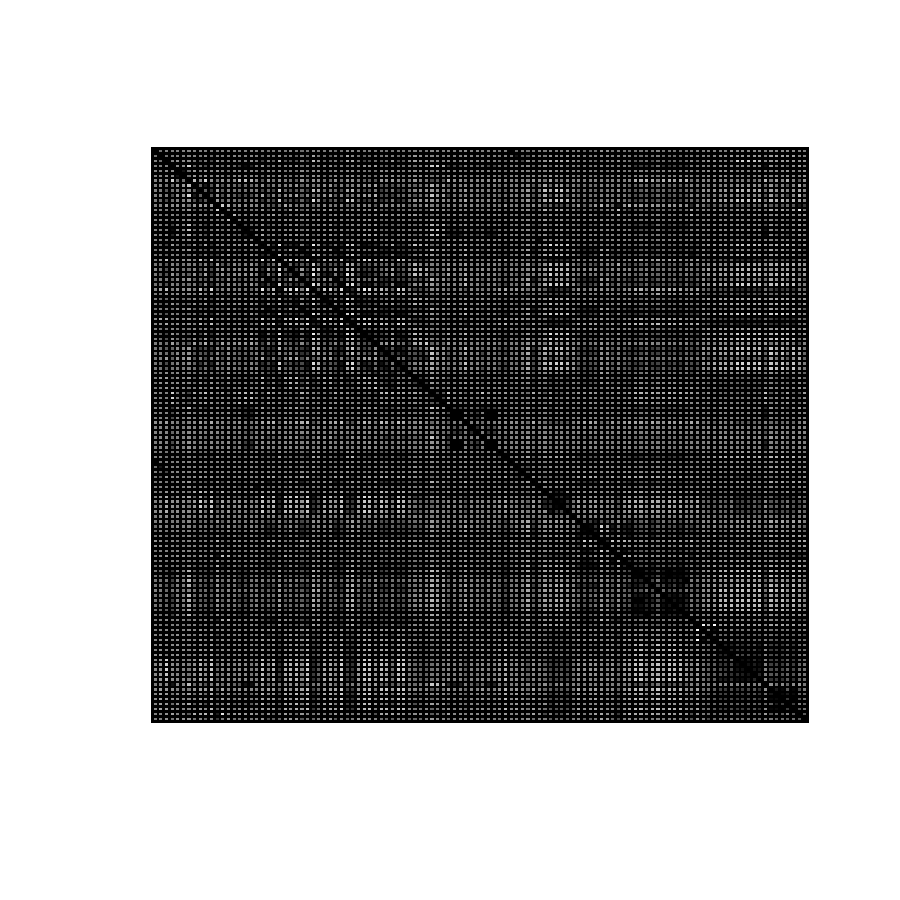
\includegraphics[width = 3.5in]{memoria-autoc}
\caption{Autocorrelació de les 117 variables.} \label{fig:autoc}
\end{figure}



\begin{figure}
\centering
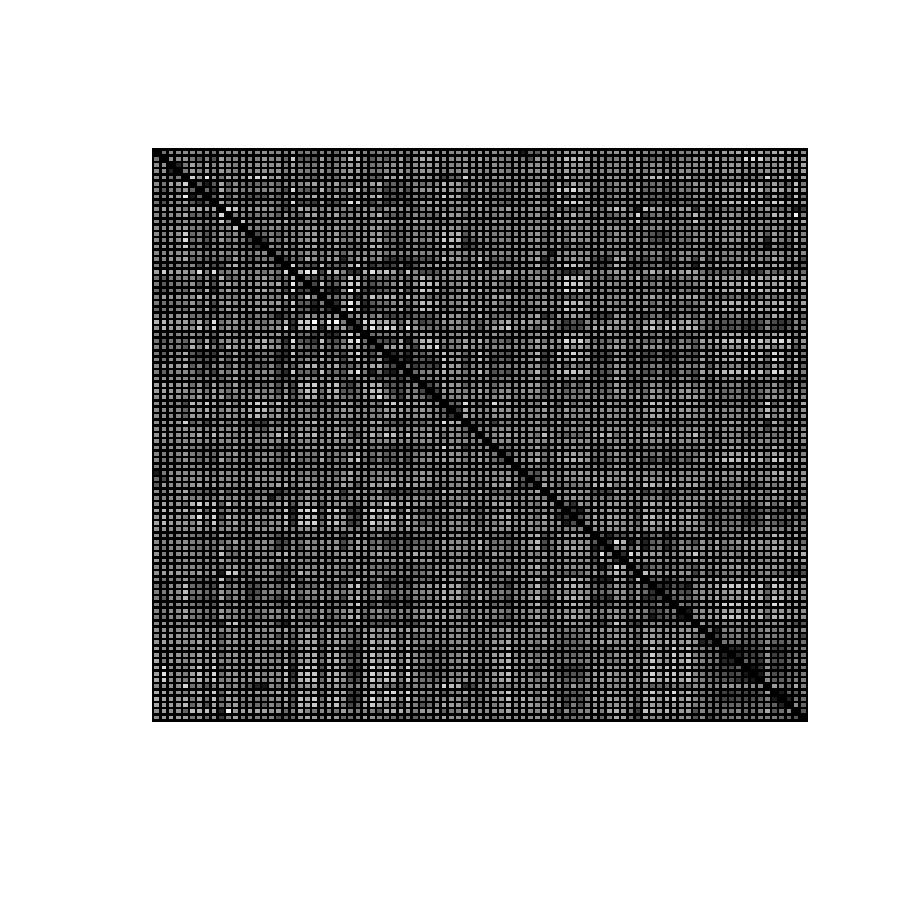
\includegraphics[width = 3.5in]{memoria-autoc_clean}
\caption{Autocorrelació de les 91
variables.} \label{fig:autoc_clean}
\end{figure}


% # <<fig=TRUE,echo=FALSE, include=FALSE, label=pos>>=
% # ggpairs(mostra.df[,c(1,v_pos,5)], colour='label')
% # @

% \begin{figure}
% \centering
% 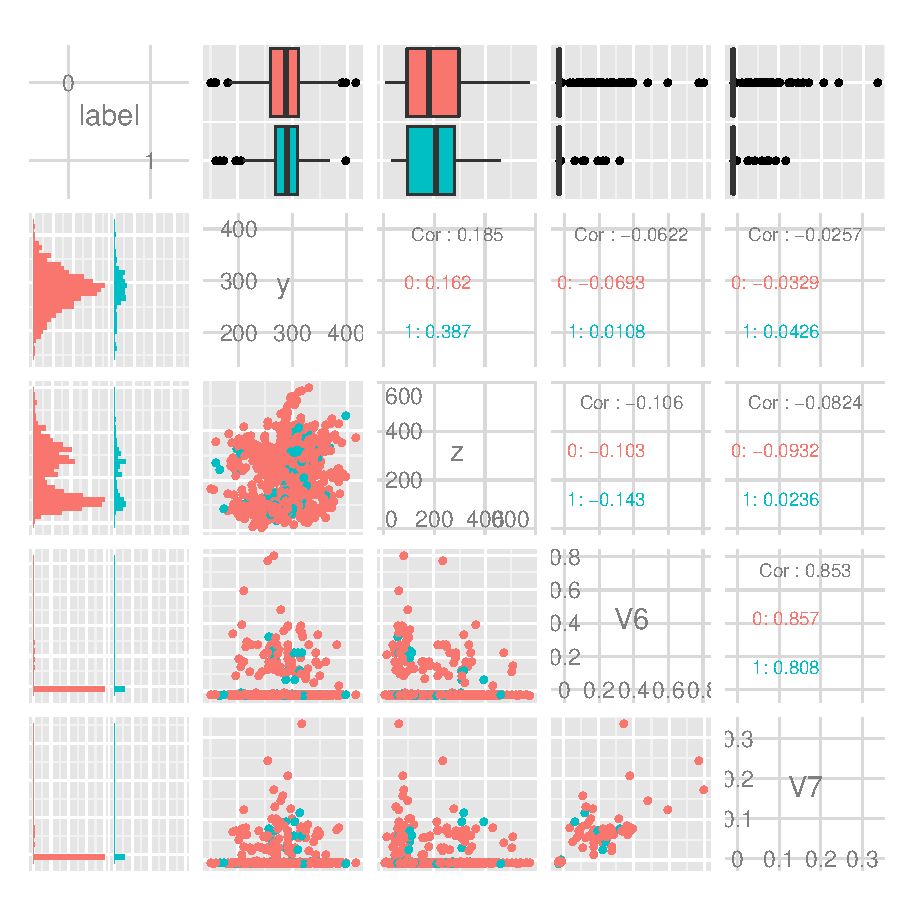
\includegraphics[width=5in]{memoria-pos}
% \caption{Scatters, distribucions condicionades, correlacions i boxplots de les variables coordenades i la mida del candidat (\texttt{V5}).} \label{fig:pos}
% \end{figure}


% # <<fig=TRUE,echo=FALSE, include=FALSE, label=top_var>>=
% # ggpairs(f_pe[,c(1,v_top)], colour='label')
% # @

% \begin{figure}
% \centering
% 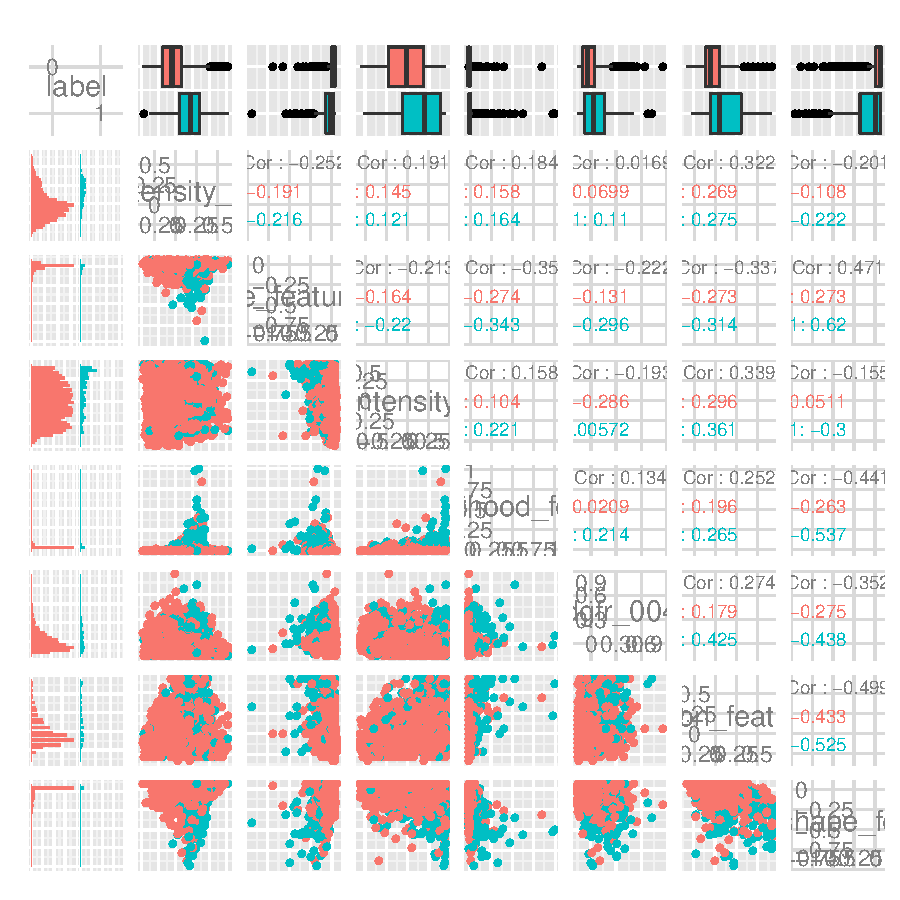
\includegraphics[width=5in]{memoria-top_var}
% \caption{Variables més importants segons el CAT score.} \label{fig:top_var}
% \end{figure}


%%%%%%%%%%%%%%%%%%%%%%%%%%%%%%%%%%%%%%%%%%%%%%%%%%%%%%%%%%%%%%%%%%%%%%%%%%%%%%%%%%%%%%%%%%%%%%%%%%%
\section{Reducció de dimensionalitat}

%%%%%%%%%%%%%%%%%%%%%%%%%%%%%%%%%%%%%%%%%%%%%%%%%%%%%%%%%%%%%%%%%%%%%%%%%%%%%%%%%%%%%%%%%%%%%%%%%%%
\section{Classificadors}
\subsection{DDA, LDA, QDA}
En aquest aprtat avaluarem els resultats dels classificadors bastats en discriminants. Concretament hem estudiar el DDA (\textit{Diagonal Discriminant Analysis} o  \textit{Naive Bayes} on la matriu de covariàncies diagonals o, equivalentment, que les variables del model són independents), el LDA i QDA. Analitzem també diversos escenaris en funció de les variables d'entrada dels models . De tots ells en donem la probabilitat d'error en el conjunt de test i conjunt d'entranament i quan és possible la curva ROC en el conjunt de test.
\\
\\
Comencem mostrant una comparativa entre els tres classificadors aplicats sobre les 91 variables (n'hem extret les no correlacionadaes tal com hem comentat en la secció de visualització de dades). En la taula \ref{tab:error_da1} podem observar els errors de classificació dels tres algorismes en els conjunts de train i test. DDA, que fa la hipotèsi més forta de independència entre les variables obté el pitjor resultat en els dos conjunts. Tant LDA com QDA obtenen errors amb ordres de magnitud similars. Tanmateix QDA sembla produir una mica més de \textit{overfitting} al tenir un error menor en el conjunt d'entrenament i un superior al de test respecte LDA. En sentit global podem dir que LDA obté millors resultats per aquest problema de QDA. 

% latex table generated in R 2.15.2 by xtable 1.7-0 package
% Sun Jan  6 20:01:08 2013
\begin{table}[ht]
\begin{center}
\begin{tabular}{rrr}
  \hline
 & error\_train & error\_test \\ 
  \hline
DDA & 0.18 & 0.22 \\ 
  LDA & 0.09 & 0.10 \\ 
  QDA & 0.07 & 0.11 \\ 
   \hline
\end{tabular}
\caption{Comparativa dels classificadors sobre les 91 variables no classificades}
\label{tab:error_da1}
\end{center}
\end{table}
En la figura \ref{fig:da_roc} hem inclòs també la curva ROC per als classificadors DDA i LDA per poder comparar-los millor. 
\\
\\
\subsubsection{Selecció i projecció de variables}
En la segona part de l'ànalisis d'aquests classificadors, hem avaluat el LDA (per ser el que millors resultats ha obtingut) per diferents conjunts de variables. Pretenm aquí veure l'efecte dels classificadors en dos nous subconjunts de variables. Per una banda, usant les variables obtingudes per PCA i ICA (projecció). Per altra, usant només aquelles variables més significatives (selecció), on ja detallarem qué entenem per més significatives.  
\\
\\
PCA i ICA
\\
\\
La segona metodologia empleada per la selecció de varibles és la de selecció de les més significatives. La selecció de variables més significatives sol ser una fase molt important en l'entrenament de classificadors per dos motius: per una banda redueix l'error de generalització i per altra disminueix el cost computacional de l'entrenament. Existeix una àmplia bibliogràfia sobre diferents metodologies de selecció de variables, tant seleccions genèriques (tipo filtres, tal com hem fet al eliminar les variables correlacionades) com seleccions espcífiques per cada classificador (\textit{wrapper}). En el nostre cas hem empleat el marc teòric del classificador LDA per puntuar cada una de les variables mitjançant els \textit{CAT scores} (una explicació detallada del mètode és pot trobar a \cite{strimmer10}). En la imatge \ref{fig:top_var_da} podem observar les 10 variables més significatives així com la magnitud de la seva importància i el signe de les seva contribució (si el seu augment contribueix a una o una altra classe). Per tal de saber quin era el nombre de varibales més adient per usar, em fet una gràfica del error comés en el test set segons els nombre usat. Aquesta gràfica (figra \ref{fig:lda_var_selec}) ens mostra que per 43 variables obtenim l'error en el test menor. A partir de llavors l'error incrementa de nou.
\\
\\
En la taula \ref{tab:error_da2} es pot veure els resultat de tots els subconjunts de variables usats: \texttt{LDA} per al classificador amb les 91 variables, \texttt{LDAPCA} i \texttt{LDAICA} per als classificadors amb variables PCA i ICA respectivament i \texttt{LDAselect} per al classificador usant només les 43 variables més importants. [ANALISIS ICA I PCA]

% latex table generated in R 2.15.2 by xtable 1.7-0 package
% Sun Jan  6 20:01:08 2013
\begin{table}[ht]
\begin{center}
\begin{tabular}{rr}
  \hline
 & error\_test \\ 
  \hline
LDA & 0.10 \\ 
  LDA\_PCA & 0.00 \\ 
  LDA\_ICA & 0.00 \\ 
  LDA\_selec & 0.10 \\ 
   \hline
\end{tabular}
\caption{Comparativa de LDA aplicat sobre diversos conjunts de variables}
\label{tab:error_da2}
\end{center}
\end{table}

\begin{figure}
\centering
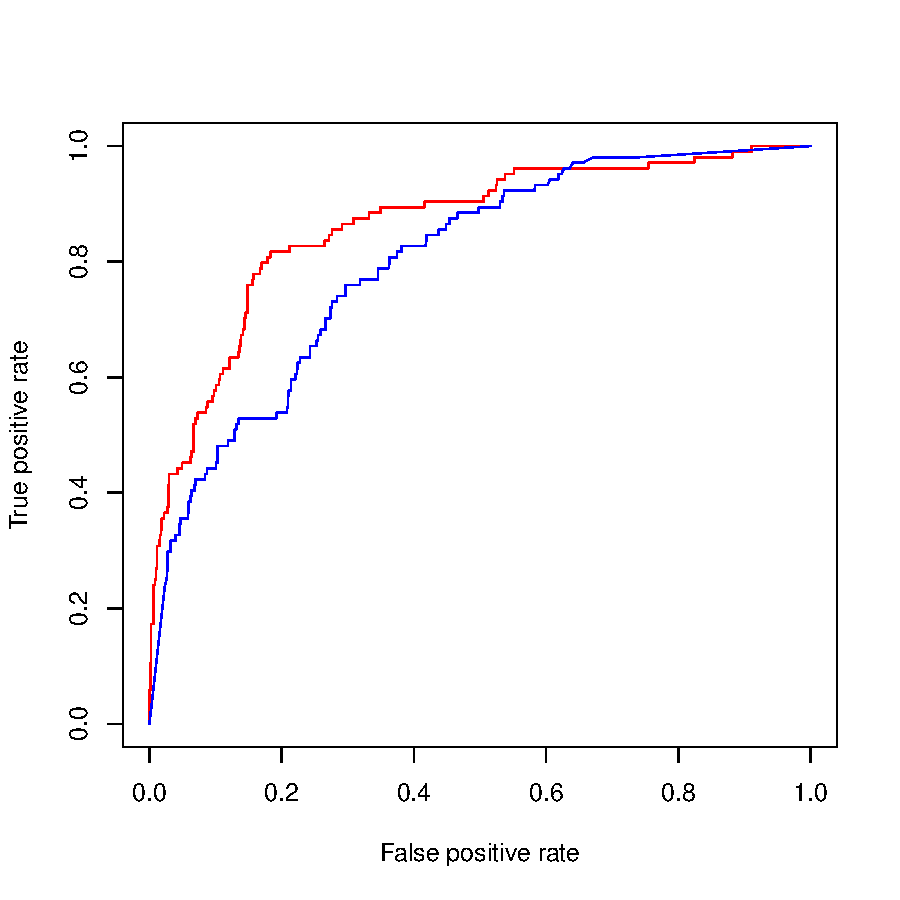
\includegraphics[width=3.5in]{memoria-da_roc}
\caption{Curva ROC de LDA (en vermell) i DDA (en blau).} \label{fig:da_roc}
\end{figure}


\begin{figure}
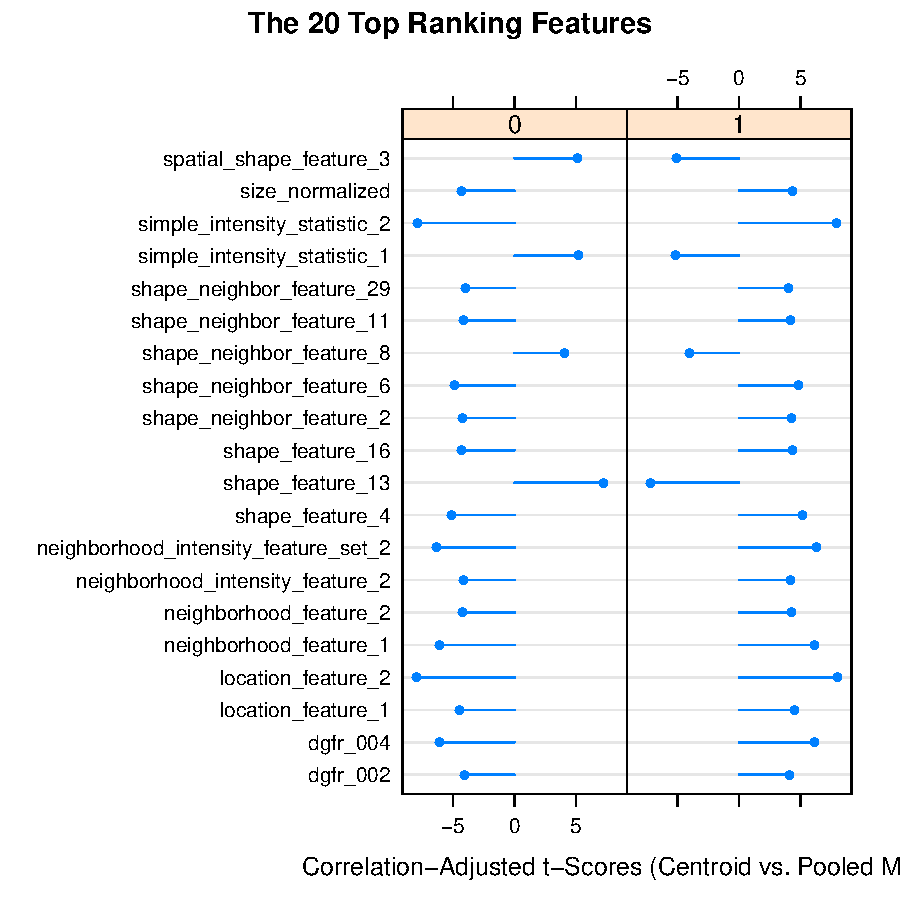
\includegraphics[width=3.5in]{memoria-top_var_da}
\caption{Ranking de les 10 variables més significatives i la seva contribució a cada una de les classes.} \label{fig:top_var_da}
\end{figure}



\begin{figure}
\centering
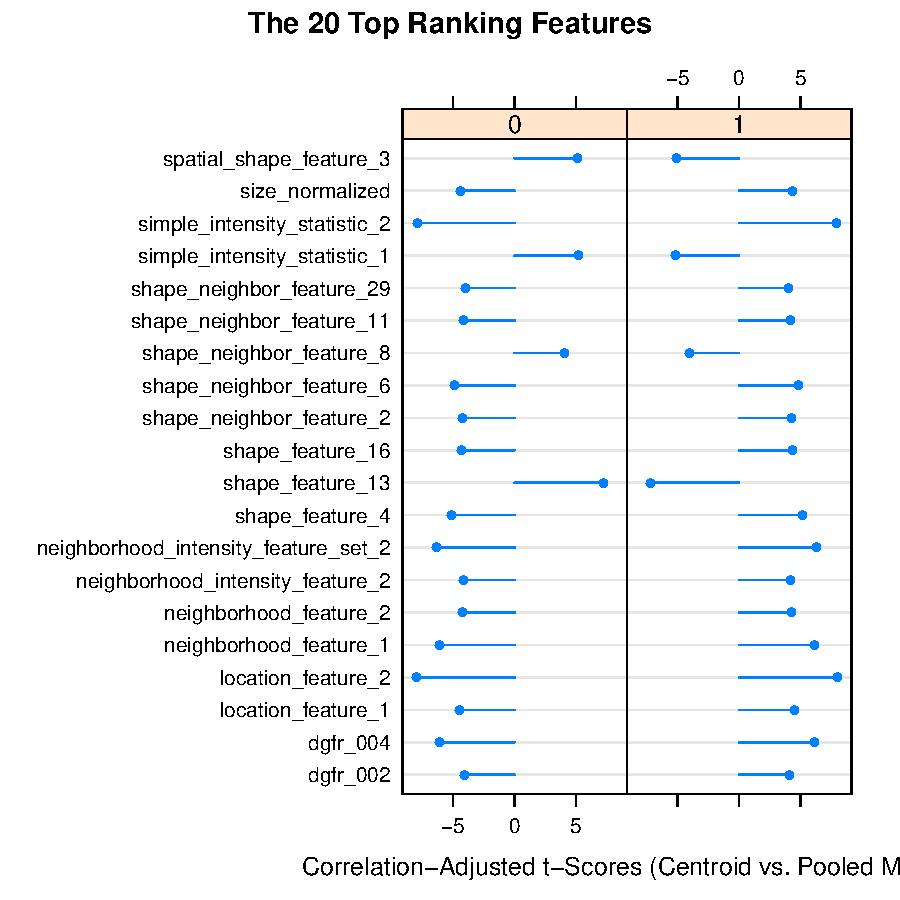
\includegraphics[width=3.5in]{memoria-lda_var_selec}
\caption{Error en el conjunt de test en funció del nombre de variables usades (oredenades segons importància de CAT score).} \label{fig:lda_var_selec}
\end{figure}

%%%%%%%%%%%%%%%%%%%%%%%%%%%%%%%%%%%%%%%%%%%%%%%%%%%%%%%%%%%%%%%%%%%%%%%%%%%%%%%%%%%%%%%%%%%%%%%%%%%

\subsection{k-NN}
\subsection{SVM}

%%%%%%%%%%%%%%%%%%%%%%%%%%%%%%%%%%%%%%%%%%%%%%%%%%%%%%%%%%%%%%%%%%%%%%%%%%%%%%%%%%%%%%%%%%%%%%%%%%%
\subsection{Xarxes Neuronals}
Presentem aquí els resutlats de l'entrenament de l'entrenament de les Xarxes Neuronals (NN). En primer lloc, hem tingut en compte la dependència de les NN respecte el seus valors inicials per lo que hem canviat el marc de treball per fer-lo més robust. Hem també  usat diferents mètodes per determinar els paràmetres òptims de les xarxes i presentem també els resultats de classificació i curves ROC per diferents conjunts de variables usats.
\\
\\
Per entrenar les xarxes neuronals hem canviat una mica el nostre marc de treball format, fins ara, per un conjunt d'entrenament i un de test. Degut a que les xarxes neuronals tenen una dependència elevada amb els seus valors inicials, hem optat per usar la tècnica de la validació creuada \textit{k-fold}. Aquesta tècnica consisteix en partir el conjunt total de dades en $k$ parts. Aleshores, s'entrena el classificador en $k-1$ i s'evalua en la restant. D'aquesta manera és pot usar el mateix conjunt de dades per obtenir fins a $k$ mesures de l'error sobre un conjunt de test. Respecte l'entrenament de les xarxes, hem seguit la filosofia general suggerida a \cite{hastie09}. Allí se'ns proposa entrenar les xarxes neuronals amb només una capa oculta. Per seleccionar el nombre de unitats d'aquesta capa, s'introdueix un terme de regularització (\textit{shrinkage}) que ens penalitza tenir molts paràmetres. Així doncs, la metodologia usada ha estat entrenar les xarxes amb 8 unitats imaginàries i determinar per validació creuada el valor òptim del terme de penalització. Aquest parametre regularitzador ja se n'encarregarà de posar a 0 les neurones de la cap intermitja que facin falta. 
\\
\\
En la figura \ref{fig:nn_regular} podem observar com varia l'error en el conjunt de test (mitja dels $k$ entrenaments) en funció del terme de regularització. En totes elles estem usant 8. Després de diverses execucions probant diferents valors, obtenim que l'ordre de magnitud del valor òptim és $10^{-2}$. Per aquests paràmetres descrits podem observar en la figura \ref{fig:nn_roc} la curva ROC per les diferents realitzacions de \textit{5-fold} validació creuada. Obtenim una mitja de 0.80 per l'AUC. Pel que fa a l'error comés l'òptim descrit obtenim 0.141 que és lleugerament més elevat que en LDA. 
\\
\\
Finalment i paral·lelament al que hem estat fent amb els altres classificadors anem a estudiar com es comporten les xarxes neuronals en funció de les variables usades. En aquest cas només mirarem l'evolució de l'error en les NN en funció del nombre de components principals usades (provinents de la projecció PCA) i en compararem el resultat amb usar totes les variables. En la figura \ref{fig:nn_princomp} podem veure l'error en el conjunt de test (després de passar per validació creuada 5-\textit{fold}) en funció del nombre de components principals usades. Podem veure que amb 7 components principals ja obtenim un error de 0.16, molt pròxim al obtingut amb les xarxes neuronals amb totes les variables (91!).



\begin{figure}
\centering
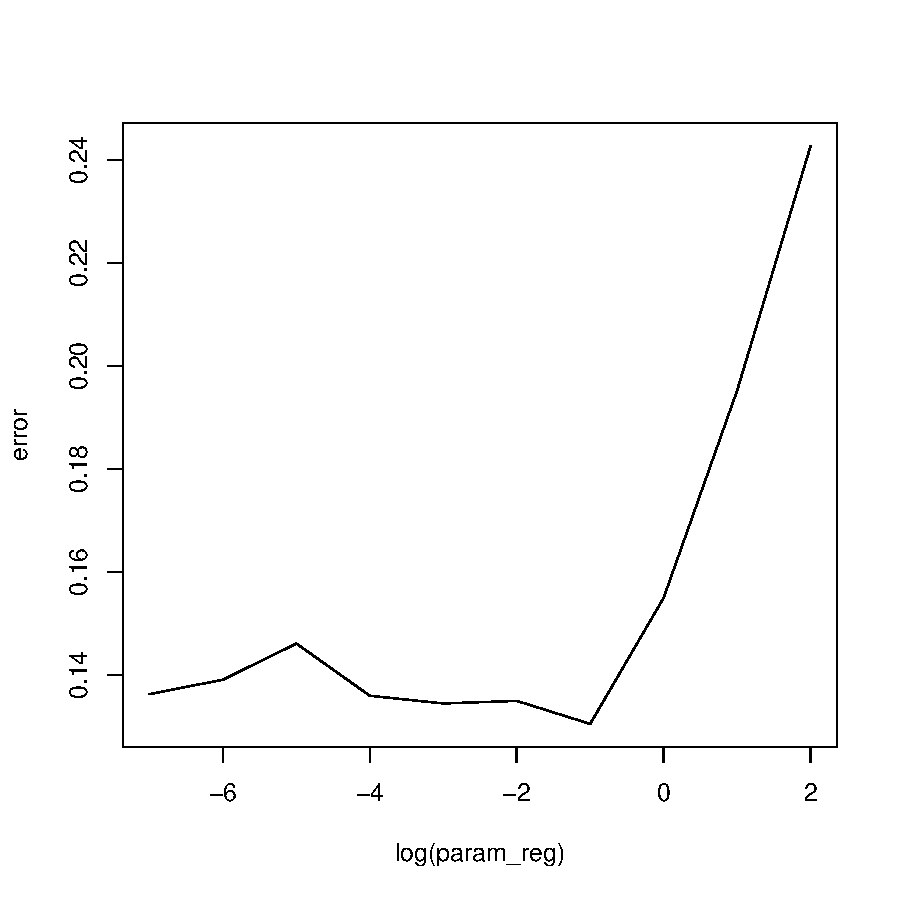
\includegraphics[width=3.5in]{memoria-nn_regular}
\caption{Error en el conjunt de test en funció del valor del paràmetre de regularització emprat en una nn d'una capa oculta i 8 unitats amagades. La variació del parametre regularitzador s'ha realitzat en escala logarítmica.} \label{fig:nn_regular}
\end{figure}


\begin{figure}
\centering
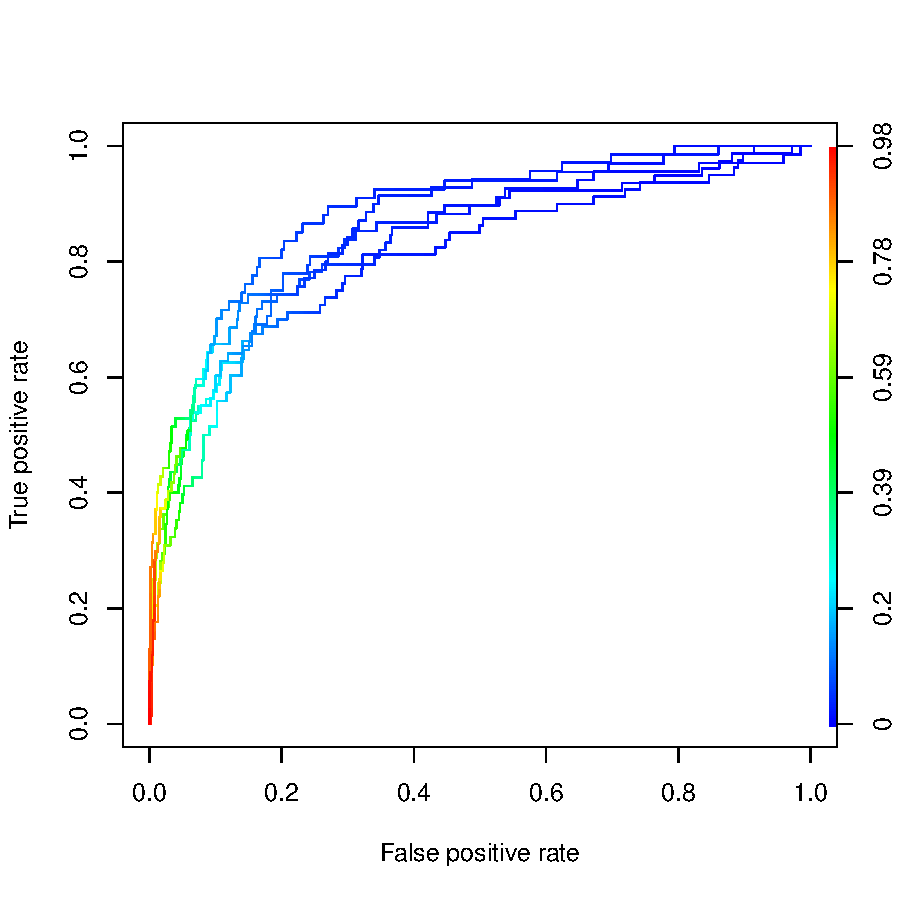
\includegraphics[width=3.5in]{memoria-nn_roc}
\caption{Curves ROC per la NN amb 8 neurones en capa oculat, amb un terme de regularizació de 0.05. S'obté una AUC mitja de 0.85.} \label{fig:nn_roc}
\end{figure}


\begin{figure}
\centering
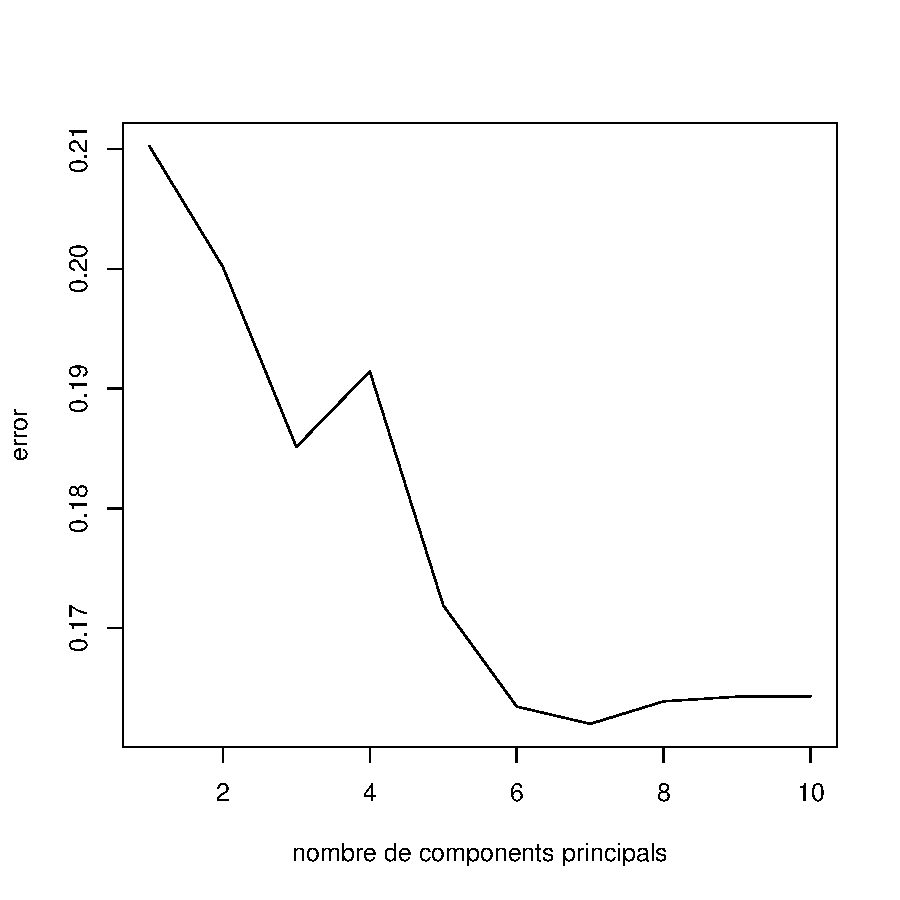
\includegraphics[width=3.5in]{memoria-nn_princomp}
\caption{Evolució de l'error en el conjunt de test en funció del nombre de components principals usades.} \label{fig:nn_roc}
\end{figure}


%%%%%%%%%%%%%%%%%%%%%%%%%%%%%%%%%%%%%%%%%%%%%%%%%%%%%%%%%%%%%%%%%%%%%%%%%%%%%%%%%%%%%%%%%%%%%%%%%%%
\subsection{Arbres}
\subsection{Random Forest (opcional)}
Els \textit{Random Forest} (RF) són uns classificadors que han guanyat molta reputació recentment degut a la seva alta precisió. En aquest apartat comencem describint-ne breument el seu funcionament. Tal com hem fet amb els altres classificadors, busquem els seus paràmetres òptims minimitzant l'error en un conjunt de test.
\\
\\
Els RF fan ús del arbres de decisió combinats a través del \textit{bagging}. L'algorisme d'aprenentatge és el següent (considerant un conjunt de $N$ exemples i $D$ variables):
\begin{enumerate}
\item Escollim un subconjunt d'entrenament (selecció aleatòria amb remplaçament) $n$ inferior al total d'exemples $N$.
\item Seleccionem aleatòriament un subconjunt de variables $d$ inferior al total $D$.
\item Amb aquests elements entrenem un arbre de decisió deixant-lo créixer fins al final (sense poda).
\item Repetim el procés per un nombre $mtree$ d'arbres.
\item Finalment, la decisió de classificació de una nova instància es pren per vot majoritari sobre tots els arbres.
\end{enumerate}
Aquest algorisme s'ajuda de l'aleatorització i combinació de classificadors (tan pel conjunt d'entrenament com per les variables usades en cadascun) per tal de millorar el compromís mitja-variància de classificació. 
\\
\\
Les dos proves que hem dut a terme per acabar de refinar els RF són precisament per a concretar el nombre de variables a usar, $d$ i el nombre d'arbres a entrenar, $mtree$. En la figura \ref{fig:rf_tuning} presentem les gràfiques de l'error en funció d'aquests dos parametres. En cada gràfica s'ha deixat estàtic el paràmetre que no s'estava estudiant \footnote{Un \textit{tunning} dels paràmetres més precís hagués estat anar iterant els resultats obtinguts simultàniament per obtenir l'òptim dels dos paràmetres a la vegada.}. En base a aquestes gràfiques hem escollit usar 17 variables i 50 arbres.
\\
\\
Finalment presentem pels valors òptims obtinguts les curves ROC després de la validació creuada \textit{k-fold} en la figura \ref{fig:rf_roc}. Els RF també ens proporcionen una mètrica de la importància de les variables que podem contrastar amb la obtinguda a través dels \textit{CAT scores} dels DA. Aquesta mètrica està basada en la impuritat de Gini. Segons aquesta, les 10 variables més importants són:
% latex table generated in R 2.15.2 by xtable 1.7-0 package
% Sun Jan  6 20:01:08 2013
\begin{table}[ht]
\begin{center}
\begin{tabular}{rlr}
  \hline
 & variable & Guany Gini \\ 
  \hline
1 & simple\_intensity\_statistic\_2 & 27.50 \\ 
  2 & size\_normalized & 20.70 \\ 
  3 & spatial\_shape\_feature\_3 & 14.93 \\ 
  4 & dgfr\_006 & 13.64 \\ 
  5 & location\_feature\_2 & 12.48 \\ 
  6 & neighborhood\_feature\_1 & 11.61 \\ 
  7 & simple\_intensity\_statistic\_1 & 11.15 \\ 
  8 & dgfr\_004 & 10.94 \\ 
  9 & location\_feature\_1 & 10.27 \\ 
  10 & neighborhood\_intensity\_feature\_set\_2 & 8.92 \\ 
   \hline
\end{tabular}
\caption{10 variables més importants segons el criteri d'impuritat de Gini extrets a partir de l'entrenament dels 	extit{random forest}}
\label{tab:topvar_gini}
\end{center}
\end{table}
\begin{figure}
\centering
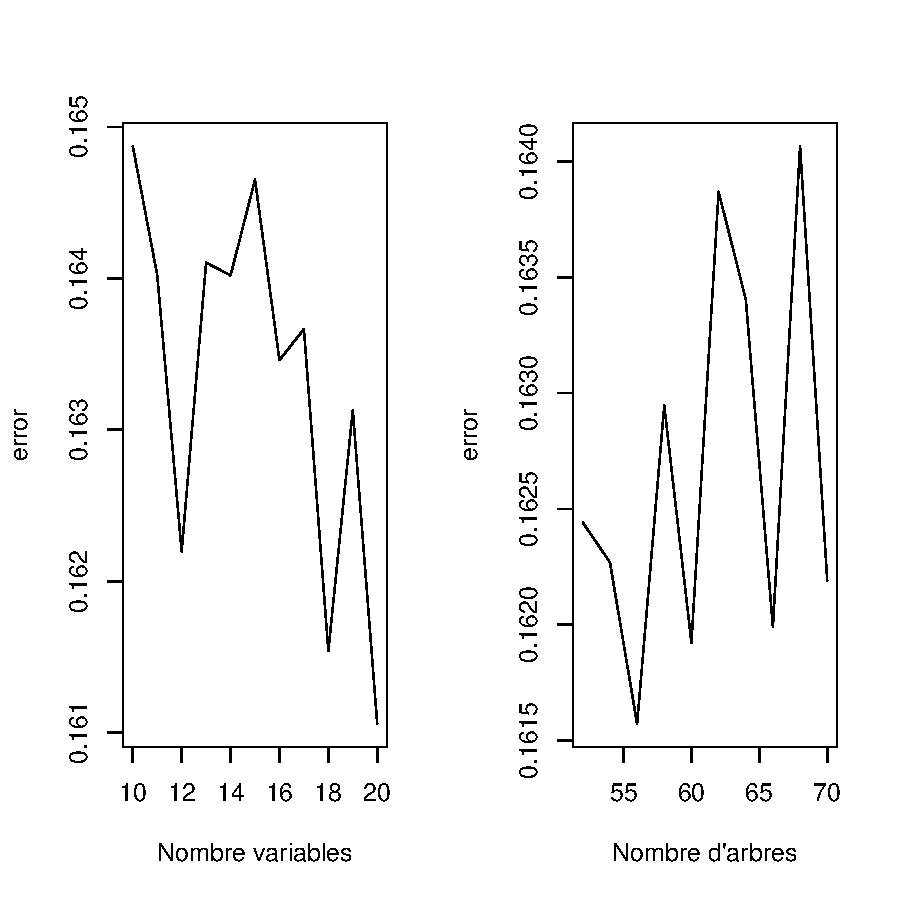
\includegraphics[width=3.5in]{memoria-rf_tuning}
\caption{Evolució de l'error en el conjunt de test en funció del nombre de components principals usades.} \label{fig:rf_tuning}
\end{figure}


\begin{figure}
\centering
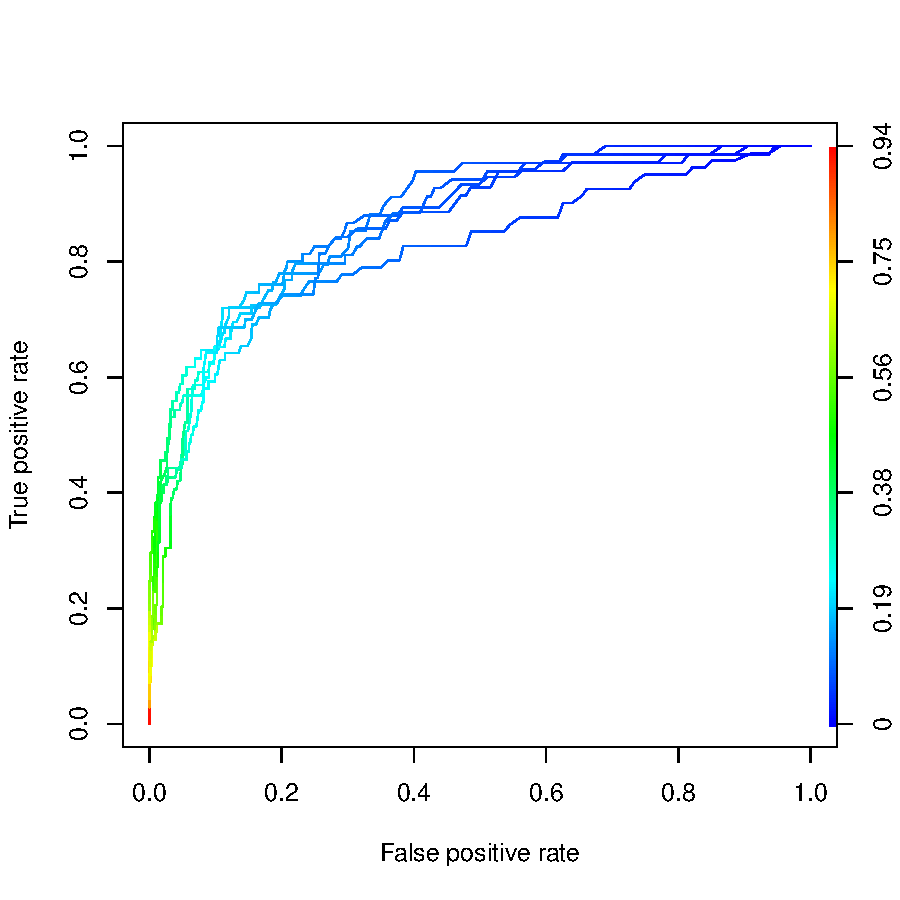
\includegraphics[width=3.5in]{memoria-rf_roc}
\caption{Curves ROC pels 5 conjunts de validació creuada per als paràmetres òptims obtinguts (17 variables per arbre i 50 arbres). Mitja AUC de 0.86.} \label{fig:rf_roc}
\end{figure}


%%%%%%%%%%%%%%%%%%%%%%%%%%%%%%%%%%%%%%%%%%%%%%%%%%%%%%%%%%%%%%%%%%%%%%%%%%%%%%%%%%%%%%%%%%%%%%%%%%%
\section{Conclusions}

%%%%%%%%%%%%%%%%%%%%%%%%%%%%%%%%%%%%%%%%%%%%%%%%%%%%%%%%%%%%%%%%%%%%%%%%%%%%%%%%%%%%%%%%%%%%%%%%%%%

\appendix
\section{Primer Apèndix}

%%%%%%%%%%%%%%%%%%%%%%%%%%%%%%%%%%%%%%%%%%%%%%%%%%%%%%%%%%%%%%%%%%%%%%%%%%%%%%%%%%%%%%%%%%%%%%%%%%%
\begin{thebibliography}{9}


\bibitem{strimmer10} %CAT scores i selecció de variables en da 
  Miika Ahdesmaki and Korbinian Strimmer,
  \emph{Feature selection in omics prediction problems using CAT scores and False Nondiscovery Rate Control},
  The Annals of Applied Statistics, 
  Vol. 4,
  2010.

\bibitem{hastie09} % neural networks
  Trevor Hastie, Robert Tibshirani, Jerome Friedman,
  \emph{The elements of statistical learning},
  Springer,
  2nd ed., 
  2009.


\end{thebibliography}

\end{document}
